\chapter{Numerické metody}
V této kapitole nejdříve popíšeme mřížkovou Boltzmannovu metodu, což je numerická metoda využitá pro simulace v této práci. Druhá část kapitoly je pak věnována poznámkám k implementaci a popisu diskretizace křivek.
\section{Mřížková Boltzmannova metoda}\label{LBM}
Mřížková Boltzmannova metoda (anglicky \textit{lattice Boltzmann method}, dále jen LBM) je numerická metoda sloužící k simulaci tekutin vyvinutá na konci dvacátého století. LBM narozdíl od jiných metod využívá tzv. mezoskopického popisu tekutiny, v kterém předpokládáme složení tekutiny z jednotlivých částic (se stejnou hmotností), jež popisujeme pomocí jednočásticových distribučních funkcí hustoty $ f(\vec{x},\vec{\xi}, t) $ \si{[kg.s^3.m^{-6}]}. Jednočásticová distribuční funkce udává hustotu částic vyskytujících se v okolí~$ \vec{x} $, v čase~$ t $ a s mikroskopickou rychlostí~$\vec{\xi}$ \cite{Kruger}. Mezoskopický popis lze chápat jako mezistupeň mezi makroskopickým popisem, který nahlíží na tekutinu jako na celek, a mezi popisem mikroskopickým, v kterém je stav systému odvozen ze znalosti stavů všech částic v něm obsažených.

Výše uvedená distribuční funkce $ f(\vec{x},\vec{\xi}, t) $ splňuje Boltzmannovu transportní rovnici
\begin{equation}\label{eq:BTR}
\frac{\partial f}{\partial t} + \sum_{i = 1}^{3} \xi _{i} \frac{\partial f}{\partial x_{i}} + \frac{1}{m} \sum_{i = 1}^{3} F_{i} \frac{\partial f}{\partial \xi _{i}} = \mathcal{C}(f), 
\end{equation}
kde $ \frac{1}{m} \vec{F} $ \si{[m.s^{-2}]} je vektor zrychlení působení vnějších sil (uvažujeme stejnou hmotnost $ m $ \si{[kg]} pro všechny částice systému) a $ \mathcal{C}(f)$ \si{[kg.s^2.m^{-6}]} je kolizní operátor, který bude více rozebrán později v sekci \ref{kol}. Boltzmannova transportní rovnice \eqref{eq:BTR} představuje fyzikální základ pro LBM. \cite{Kruger}

Numerické schéma LBM můžeme odvodit pomocí diskretizace Boltzmannovy transportní \ rovnice~\eqref{eq:BTR}. Diskretizace prostoru je provedena pomocí ekvidistantní mřížky (anglicky \textit{lattice}).
%, na které jsou diskrétně rozloženy uvažované částice tekutiny.
%Uvažujeme mřížku, jejíž všechny sousední uzly jsou od sebe vzdáleny stejně, mřížka je tedy ekvidistantní.
Diskretizace prostoru rychlostí se odvíjí od volby rychlostního modelu, který označujeme D$d$Q$q$, kde $ d$ a $q $ značí dvě hlavní charakteristiky:
\begin{itemize}
	\item[] $ d $ - dimenzi uvažovaného prostoru,
	\item[] $ q $ - počet navzájem různých směrů, podél nichž se může informace po mřížce šířit.
\end{itemize}
Každému z možných směrů pohybu pak přísluší diskrétní distribuční funkce hustoty \mbox{$ f_{i}, \ i \in \{0,\dots, q-1 \}$}. Příklady některých používaných rychlostních modelů v různých dimenzích jsou k nahlédnutí na obr. \ref{fig:lattice}. V~této práci budeme uvažovat rychlostní model D2Q9.
\begin{figure}[h]
	\centering
	\begin{subfigure}{0.88\textwidth}
		\centering
		\includegraphics[width=.7\textwidth]{Images/d1q3.pdf}
		\caption{D1Q3}
		\label{fig:lattice1}
	\end{subfigure}%
	\\[20pt]
	\begin{subfigure}{0.88\textwidth}
		\centering
		\includegraphics[width=.71\textwidth]{Images/d2q9.pdf}
		\caption{D2Q9}
		\label{fig:lattice2}
	\end{subfigure}
	\vspace{3mm}
	\caption{Příklady rychlostních modelů pro jednu a dvě dimenze.}
\label{fig:lattice}
\end{figure}
\subsection{Bezrozměrné jednotky}\label{jednot}
Pro diskretizaci rovnice \eqref{eq:BTR} je výhodné přejít od fyzikálních jednotek k jednotkám bezrozměrným, ve kterých následně probíhají simulace LBM. Jak již bylo zmíněno, k diskretizaci je využita pravidelná mřížka, bezrozměrné jednotky proto v našem případě budeme nazývat mřížkové jednotky (anglicky \textit{lattice units}). Postupně popíšeme konverzní vztahy mezi fyzikálními a mřížkovými jednotkami pro prostorový krok $\Delta l$ \si{[m]}, časový krok $\Delta t$ \si{[s]}, složky rychlosti $u_{i}$ \si{[m.s^{-1}]} a kinematickou viskozitu $\nu$ \si{[m^{2}.s^{-1}]}. Všechny veličiny v mřížkových jednotkách budeme dále značit pravým horním indexem $ L $.

Zdůrazněme, že fyzikální principy jsou nezávislé na volbě soustavy jednotek. Pro konzistentní přechod k bezrozměrným jednotkám je nutné dodržet zákon podobnosti pro dynamiku tekutin, viz \cite{Landau}. Dle něj jsou dva systémy ekvivalentní, je-li zachována velikost relevantních bezrozměrných veličin, mezi něž patří např. Reynoldsovo číslo, které je definováno vztahem
\begin{equation}\label{Re}
\mathrm{Re} = \dfrac{l_{0} u_{0}}{\nu} = \dfrac{l^{2}_{0}}{t_{0} \nu},
\end{equation}
kde $ \nu $ je kinematická viskozita a dále $ l_{0} $~\si{[m]}, $ t_{0} $ \si{[s]} a $ u_{0} $~\si{[m.s^{-1}]} jsou po řadě charakteristická délka, charakteristický čas a charakteristická rychlost \cite{Landau}. Hodnoty těchto veličin volíme v souladu s danou fyzikální úlohou. Jako $ l_{0} $ nejčastěji volíme rozměr výpočetní oblasti, $ u_{0} $ je pak typicky maximální či průměrná rychlost tekutiny v oblasti \cite{Kruger}. Pro $ t_{0} $ platí vztah
\begin{equation}
t_{0} = \dfrac{l_{0}}{u_{0}}.
\end{equation}
Konverzní vztahy pro $\Delta l^{L}$ \si{[-]}, respektive $\Delta t^{L}$~\si{[-]} mají následující podobu:
\begin{subequations}\label{conv1}
	\begin{eqnarray}
	\Delta l = \dfrac{l_{0}}{{l^{L}_0}}\Delta l^{L},\\[5pt]
	\Delta t = \dfrac{t_{0}}{{t^{L}_0}}\Delta t^{L}.
	\end{eqnarray}
\end{subequations}
Pro zjednodušení se často pokládá $ \Delta l^{L} = \Delta t^{L} = 1 $, viz \cite{Kruger}, poté vztahy \eqref{conv1} přejdou v
\begin{subequations}\label{conv2}
	\begin{eqnarray}
	l^{L}_0 = \dfrac{l_{0}}{\Delta l},\\[5pt]
	t^{L}_0 = \dfrac{t_{0}}{\Delta t},
	\end{eqnarray}
\end{subequations}
což jsou převodní vztahy, které jednoznačně určují charakteristickou délku a charakteristický čas v LBM.
S využitím vztahů \eqref{conv2} lze odvodit převodní vztah pro složky rychlosti ve tvaru
\begin{equation}\label{conv_v}
u_{i} = \dfrac{\Delta l}{\Delta t} u^{L}_{i}, \ i \in \{1, 2, 3\},
\end{equation}
kde $ u^{L}_{i} $ značí složky vektoru bezrozměrné rychlosti.
%Jak již bylo zmíněno, při přechodu od fyzikálních jednotek k mřížkovým jednotkám požadujeme, aby byla zachována mimo jiné velikost Reynoldsova čísla, což je bezrozměrná veličina, která je definovaná vztahem

Z podmínky zachování velikosti $ \mathrm{Re} $ při přechodu mezi soustavami v kombinaci s již zmiňovanou volbou $ \Delta l^{L} = \Delta t^{L} = 1 $ pak plyne konverzní vztah pro $ \nu $ ve tvaru
\begin{equation}\label{nu}
\nu = \dfrac{\Delta l^{2}}{\Delta t} \nu^L.
\end{equation}
Ze vztahu \eqref{nu} můžeme vidět, že pro danou síť s prostorovým krokem $ \Delta l $ je časový krok $ \Delta t $ svázán s~hodnotou $ \nu^L $.


V této kapitole budeme dále pracovat výhradně s veličinami v mřížkových jednotkách, upustíme tedy od rozlišování pomocí speciálního označení a nebudeme používat horní index $ L $, ačkoliv budeme bezrozměrný popis uvažovat. Pokud to bude kontext vyžadovat, odlišíme dále veličiny ve fyzikálních jednotkách horním indexem $ F$.

\subsection{Definice a diskretizace výpočetní oblasti}\label{disk}
Výpočetní oblast v této práci bude představovat oblast $ \Omega  \subset \mathbb{R}^3$. Těleso umístěné ve výpočetní oblasti budeme \mbox{značit $ \Omega_{\mathrm{b}} $.} Platí tedy $ \Omega_{\mathrm{b}} \subset \Omega$. Časový interval, na kterém budeme úlohu vyšetřovat budeme značit $ \mathcal{I} $, přičemž $ \mathcal{I} = \langle 0, T \rangle \subset \mathbb{R},$ kde $ T > 0$. Veškeré vztahy popisující dynamiku tekutin v kapitole \ref{mmodel} jsou platné v $ \mathbb{R}^3 $, nicméně v rámci této práce budeme jeden z rozměrů uvažovat jako jednotkový a omezíme se tak pouze na 2D úlohy. Platnost rovnic popisujících dynamiku tekutin však zůstává nezměněna. Hranici oblasti $ \Omega $ budeme značit $ \partial \Omega $ a budeme ji vnímat jako uzávěr disjunktního sjednocení jednotlivých částí hranice, viz obr. \ref{fig:vypocetni-oblast}.

Konkrétně rozdělíme hranici jako
\begin{equation}\label{eq:border decomposition}
\partial \Omega = \overline{\partial \Omega_{\mathrm{in}} \cup \partial \Omega_{\mathrm{out}} \cup \partial \Omega_{\mathrm{wall}}},
\end{equation}
přičemž platí, že
\begin{equation}
\partial \Omega_{\mathrm{in}} \cap \partial \Omega_{\mathrm{out}} \cap \partial \Omega_{\mathrm{wall}} = \emptyset.
\end{equation}
\begin{figure}[h]
	\centering
	\vspace{-3.8mm}
	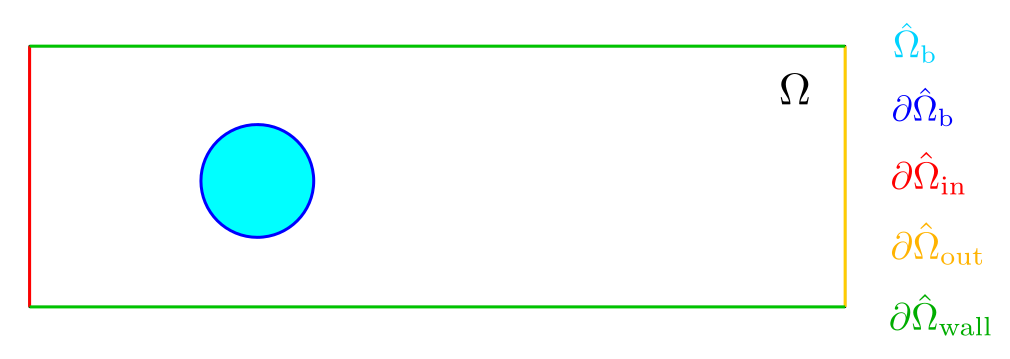
\includegraphics[width=1.0\textwidth]{Images/vypocetni-oblast.pdf}
	\vspace{-3.8mm}
	\caption{Definice výpočetní oblasti $ \Omega $, jejíž hranice $ \partial \Omega $ je disjunktně rozdělena na tři části $ \partial \Omega _{\mathrm{in}} $, $ \partial \Omega _{\mathrm{out}} $ a $ \partial \Omega _{\mathrm{wall}} $. V oblasti se dále nachází těleso $ \Omega _{\mathrm{b}} $ s hranicí $ \partial \Omega _{\mathrm{b}} $.}
	\label{fig:vypocetni-oblast}
\end{figure}

Diskretizaci výpočetní oblasti $ \Omega $ provedeme pomocí ekvidistantní izotropické mřížky ve tvaru
\begin{subequations}\label{eq:oblast}
	\begin{eqnarray}
	\hat{\Omega} &=& \big\{ \vec{x}_{i,j} = (i \Delta l,\,j \Delta l)^T \, \textbar \ i \in \{1, \dots, N_{x} - 1\}, j \in \{1, \dots, N_{y} - 1 \} \, \big\},\\[4pt]
	\overline{\hat{\Omega}} &=& \big\{ \vec{x}_{i,j} = (i \Delta l,\,j \Delta l)^T \, \textbar \ i \in \{0, \dots, N_{x} \}, j \in \{0, \dots, N_{y} \} \, \big\},
	\end{eqnarray}
\end{subequations}
kde $ \Delta l $ je prostorový krok. Množinu uzlů diskretizujících hranici výpočetní oblasti zavádíme jako
\begin{equation}\label{eq:border}
\partial\hat{\Omega} = \overline{\hat{\Omega}} \, \backslash \, \hat{\Omega},
\end{equation}
a obdobně jako v \eqref{eq:border decomposition} pro ni budeme uvažovat tvar
\begin{equation}\label{eq:discrete border decomposition}
\partial \hat{\Omega} = \partial \hat{\Omega}_{\mathrm{in}} \cup \partial \hat{\Omega}_{\mathrm{out}} \cup \partial \hat{\Omega}_{\mathrm{wall}},
\end{equation}
viz obr. \ref{fig:diskretni-oblast}.
\begin{figure}[H]
	\centering
	\vspace{-.4mm}
	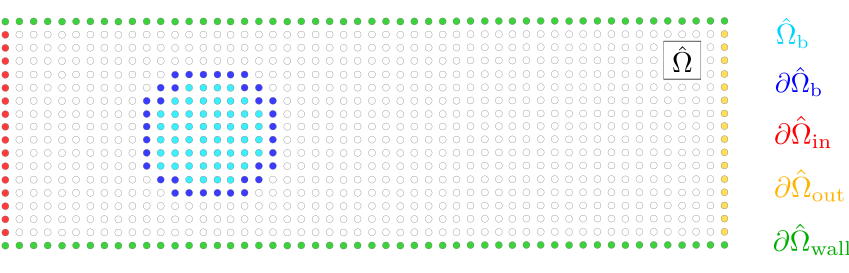
\includegraphics[width=1.0\textwidth]{Images/diskretni-oblast.pdf}
	\vspace{-3.8mm}
	\caption{Definice diskretizované výpočetní oblasti $ \hat{\Omega} $, jejíž hranice $ \partial \hat{\Omega}$ je disjunktně rozdělena na tři části $ \partial \hat{\Omega}_{\mathrm{in}} $, $ \partial \hat{\Omega}_{\mathrm{out}} $ a $ \partial \hat{\Omega}_{\mathrm{wall}} $. V oblasti se dále nachází diskretizovaná oblast reprezentující těleso $ \hat{\Omega}_{\mathrm{b}} $ s~hranicí $ \partial \hat{\Omega}_{\mathrm{b}} $.}
	\label{fig:diskretni-oblast}
	\vspace{1.8mm}
\end{figure}

Dále definujeme časový krok
\begin{equation}\label{eq:timestep}
\Delta t = \frac{T}{N_{t}}, \ N_{t} \in \mathbb{N}
\end{equation}
a časový interval $ \mathcal{I} $ diskretizujeme jako
\begin{equation}\label{eq:timediscrete}
\hat{\mathcal{I}} = \big\{ t_{i} = i \Delta t \, \textbar \ i \in \{0, \dots, N_{t} - 1\} \big\}.
\end{equation}
Diskretizací získáme diskrétní formu rovnice \eqref{eq:BTR} ve tvaru
\begin{equation}\label{eq:BTRdiscrete}
f_{k}\left(\vec{x}+\Delta t \vec{\xi}_{k}, t+\Delta t \right) =
f_{k}(\vec{x}, t) + \mathcal{C}_{k}(\vec{x}, t) + \mathcal{S}_{k}(\vec{x}, t), \hspace{2.5mm} k \in \{0, \dots, q-1 \}, \ \forall \vec{x} \in \hat{\Omega}, \ \forall t \in \hat{\mathcal{I}},
\end{equation}
kde $ \mathcal{C}_{k} $ je diskrétní kolizní operátor a $ \mathcal{S}_{k} $ je diskrétní silový člen, jejichž podoba závisí na zvoleném typu mřížkové Boltzmannovy metody \cite{Kruger}. Rovnice \eqref{eq:BTRdiscrete} se nazývá mřížková Boltzmannova rovnice (anglicky \textit{lattice Boltzmann equation}).

Po zavedení tzv. postkolizní distribuční funkce $ f^{*}_{k} $ vztahem
\begin{equation}\label{eq:fstar}
f^{*}_{k}(\vec{x}, t) = f_{k}(\vec{x}, t) + \mathcal{C}_{k}(\vec{x}, t) + \mathcal{S}_{k}(\vec{x}, t), \hspace{2.5mm} k \in \{0, \dots, q-1 \}, \ \forall \vec{x} \in \hat{\Omega}, \ \forall t \in \hat{\mathcal{I}},
\end{equation}
můžeme rovnici \eqref{eq:BTRdiscrete} přepsat ve tvaru
\begin{equation}\label{eq:collision}
f_{k}\left(\vec{x}+\Delta t \vec{\xi}_{k}, t+\Delta t\right) = f^{*}_{k}(\vec{x}, t), \hspace{2.5mm} k \in \{0, \dots, q-1 \}, \ \forall \vec{x} \in \hat{\Omega}, \ \forall t \in \hat{\mathcal{I}}.
\end{equation}
Počáteční a okrajové podmínky budou dále podrobně rozebrány v sekci \ref{initial conditions}, resp. v sekci \ref{boundary conditions}.
\subsection{Makroskopické veličiny}\label{macro}
Nyní představíme vztahy pro výpočet některých makroskopických veličin jako je hustota $ \rho $ a makroskopická rychlost $ \vec{u} $. Výpočtu tlaku je pak věnována následující sekce. Vztahy pro výpočet těchto veličin lze odvodit pomocí obecných momentů diskrétních distribučních funkcí a mají tvar

\begin{subequations}\label{macroeq}
	\begin{eqnarray}
	\label{rho}
	\rho &=& \sum_{k=0}^{q-1} f_{k},\\[3pt]
	\rho \vec{u} &=& \sum_{k=0}^{q-1} f_{k} \vec{\xi_{k}} + \dfrac{\Delta t}{2} \vec{g},
	\end{eqnarray}
\end{subequations}
kde $\vec{g}$ je diskrétní silový člen. Popis výpočtu makroskopických veličin je uveden např. v \cite{Kruger}. Tyto vztahy jsou pak v jednom z kroků algoritmu LBM použity pro výpočet a aktualizaci hodnot makroskopických veličin, viz sekce \ref{algo}.
\subsubsection{Tlak v LBM}\label{pressureLBM}
Pomocí zákona podobnosti lze ukázat, že rovnice udávající vztah pro výpočet tlaku při přechodu k mřížkovým jednotkám nabývá stejného tvaru jako v \eqref{pressure}. Pro výpočet tlaku můžeme psát
\begin{equation}\label{tlakLBM}
p = c^2_{s}\ \rho,
\end{equation}
přičemž v námi uvažovaném modelu D2Q9 platí $ c_{s} = \frac{1}{\sqrt{3}}$.

Získali jsme tedy vztah pro výpočet tlaku v~bezrozměrných jednotkách, nicméně z rovnic \eqref{NS} v~kombinaci s předpokladem izotermálního systému vyplývá, že pro naše výpočty je relevantní pouze gradient tlaku.

Nyní popíšeme, jak výpočty tlaku ze simulace spojit se skutečnou celkovou fyzikální hodnotou tlaku. Nejdříve provedeme rozklad bezrozměrné hustoty ve tvaru
\begin{equation}\label{density decomposition}
	\rho  = \rho _0 + \rho \textit{\textquotesingle},
\end{equation}
kde $ \rho_0 $ značí v čase průměrnou hodnotu hustoty $ \rho $ a $ \rho \textit{\textquotesingle} $ je v čase proměnná odchylka od průměru (fluktuace). Zdůrazněme, že ačkoliv v našem modelu uvažujeme nestlačitelnou tekutinu, hodnota LBM hustoty $ \rho $ se může z principu mřížkové Boltzmannovy metody měnit, proto má tato dekompozice smysl. Pro fyzikální hodnotu tlaku provedeme obdobnou dekompozici ve tvaru
\begin{equation}\label{pressure decomposition}
p^{F} = p_0^{F} + p\textit{\textquotesingle}^{\,F},
\end{equation}
kde opět $ p_0^F $ značí průměrnou hodnotu tlaku ve fyzikálních jednotkách a $ p\textit{\textquotesingle}^{\,F} $ je v čase proměnná odchylka od průměrné hodnoty (fluktuace). Vyjádříme nyní $ p\textit{\textquotesingle}^{\,F} $ vztahem
\begin{equation}\label{pressure devation}
p\textit{\textquotesingle}^{\,F} = K_{p} \, c^{2}_{s}\ \rho \textit{\textquotesingle},
\end{equation}
kde člen $ K_{p} $ představuje konverzní faktor pro tlak při přechodu k fyzikálním jednotkám, pro který platí vztah
\begin{equation}\label{cp}
K_{p} = \rho^{F} \ {\Big( \dfrac{\Delta l^{F}}{\Delta t^{F}} \Big)}^2,
\end{equation}
kdy uvažujeme již zmiňovanou volbu $ \Delta l = \Delta t = 1 $.

Celkem pak tedy můžeme tlak ve fyzikálních jednotkách vyjádřit jako
\begin{equation}\label{total pressure}
p^F = p^F_0 + \rho^F \ {\, \Big(c_{s} \: \dfrac{\Delta l^F}{\Delta t^F} \,\Big)}^2 \rho \textit{\textquotesingle},
\end{equation}
kde $ \rho \textit{\textquotesingle} $ získáme pomocí \eqref{density decomposition}. Tímto dostáváme možnost počítat hodnotu tlaku ve fyzikálních jednotkách. Znovu však upozorněme, že stěžejní je hodnota gradientu tlaku, a že hodnota parametru $ p^F_0 $ představující referenční hodnotu tlaku výpočty v LBM nijak neovlivňuje. Celý postup je detailně popsán~v~\cite{Kruger}.

\subsection{Kolizní operátory}\label{kol}
V LBM existuje několik způsobů, jak zavést diskrétní kolizní operátor. Tyto různé varianty aproximace pak dávají za vznik různým typům LBM, mezi něž patří například SRT-LBM~\cite{GeierCuLBM}, MRT-LBM~\cite{MRT}, CLBM~ \cite{GeierCLBM}, ELBM~\cite{ELBM} nebo CuLBM~\cite{GeierCuLBM}. V této práci se omezíme pouze na využití typu CLBM, pro úplnost však rozebereme i typ SRT-LBM, který vychází přímo z Bhatnagarova–Grossova–Krookova (BGK) spojitého fyzikálního modelu \cite{Kruger}.
\subsubsection{SRT-LBM}\label{SRT}
Jako první uvedeme variantu SRT-LBM (z anglického \textit{Single Relaxation Time}), která patří k nejjednodušším ze všech typů LBM. Použitá aproximace má tvar
\begin{equation}\label{eq:srt}
C^{SRT}_{k}(\vec{x}, t) = -  \frac{\Delta t}{\tau}(f_{k}´(\vec{x}, t) - f^{\mathrm{eq}}_{k}(\vec{x}, t)), \hspace{3mm} k \in \{1, 2, \dots, q-1\},
\end{equation}
kde $ \tau $ je relaxační čas, který vyjadřuje, jak rychle systém spěje do lokální rovnováhy \cite{GeierCuLBM}. Ta je určená pomocí rovnovážné distribuční funkce $ f^{\mathrm{eq}}_{k} $ a představuje stav, kdy se lokální veličiny v čase nemění.

Relaxační čas $ \tau $ je svázán s kinematickou viskozitou $ \nu $ vztahem
\begin{equation}\label{eq:tausrt}
\nu = c^{2}_{s} \, \Bigg( \tau - \frac{\Delta t}{2} \Bigg).
\end{equation}
V SRT-LBM můžeme silový člen $ S_{k} $ aproximovat jako
\begin{equation}\label{eq:silasrt}
S_{k} = w_{k }\Delta t \, \Bigg( 1 - \frac{\Delta t}{2\tau} \Bigg) \, \Bigg( \frac{\vec{\xi}_{k} - \vec{u}}{c^{2}_{s}} + \frac{\vec{\xi}_{k} \cdot \vec{u}}{c^{4}_{s}} \vec{\xi}_{k} \Bigg) \cdot \vec{g},
\end{equation}
kde $ w_{k } $ jsou váhy specifické pro daný rychlostní model \cite{Kruger}.
\subsubsection{CLBM}\label{CLBM}
Jako druhý typ uvedeme Centrální LBM (CLBM, anglicky \textit{Central LBM}). Narozdíl od SRT-LBM využívá CLBM celkem $ q $ relaxačních časů. Také kolizní krok je v CLBM realizován jinak - ke kolizi zde dochází v prostoru centrálních momentů distribučních funkcí $ f_{k} $. 

Omezíme se pro názornost a jednoduchost zápisu pouze na rychlostní model D2Q9. Definujme dále multiindex $ \vec{\alpha} = (\alpha_{1}, \alpha_{2}) \in \mathbb{N}^2_{0}$. Centrální momenty definujeme vztahem
\begin{equation}\label{eq:centralmoment} k_{(\alpha_{1}, \alpha_{2})} = \sum_{k=0}^{8} f_{k} (\xi_{k,1}  - u_{1})^{\alpha_{1}} (\xi_{k,2}  - u_{2})^{\alpha_{2}},
\end{equation}
kde $ \vec{u} = (u_1, u_2)^T$ je makroskopická rychlost.
%Dále definujme obecné momenty (anglicky \textit{raw moment}) jako
%\begin{equation}\label{eq:rawmoment}
%m_{\alpha_{1}, \alpha_{2}} = \sum_{k=0}^{q-1} f_{k} \xi^{\alpha_{1}}_{k,1} \xi^{\alpha_{2}}_{k,2}.
%\end{equation}

Označme dále $ \vec{f} = \left(f_{0}, f_{1}, \dots, f_{8} \right)^T$ a $ \vec{f}^{\mathrm{eq}}= \left(f^{\mathrm{eq}}_{0}, f^{\mathrm{eq}}_{1}, \dots, f^{\mathrm{eq}}_{8} \right)^T $.
Postkolizní distribuční funkci můžeme pak vyjádřit vztahem
\begin{equation}\label{eq:srt_f}
\vec{f}^{*}(\vec{x}, t) = \vec{f}(\vec{x}, t) + \mathbf{K^{-1}}\mathbf{S}\mathbf{K} (\vec{f}^{\mathrm{eq}}(\vec{x}, t) - \vec{f}(\vec{x}, t)),
\end{equation}
kde $ \mathbf{K} $ je matice přechodu z prostoru distribučních funkcí do prostoru centrálních momentů a dále matice $ \mathbf{S} $ je diagonální ve tvaru
\begin{equation}\label{eq:srt_matrixS}
\mathbf{S} = \mathrm{diag} \, \Bigg( \frac{\Delta t}{\tau_{0}}, \frac{\Delta t}{\tau_{1}}, \dots, \frac{\Delta t}{\tau_{8}} \Bigg),
\end{equation}
pro relaxační časy $ \tau_{i}, \ i \in \{0, 1, \dots, 8\}$.

Matici přechodu $ \mathbf{K} $ volíme tak, aby platilo
\begin{equation}\label{eq:srt_matrixK}
\vec{\kappa} = \mathbf{K} \vec{f} =
\begin{pmatrix}
k_{(0,0)} \\
k_{(1,0)} \\
k_{(0,1)} \\
k_{(1,1)} \\
k_{(2,0)} + k_{(0,2)} \\
k_{(2,0)} - k_{(0,2)} \\
k_{(2,1)} \\
k_{(1,2)} \\
k_{(2,2)}
\end{pmatrix}
=
\begin{pmatrix}
\rho \\
0 \\
0 \\
k_{(1,1)} \\
k_{(2,0)} + k_{(0,2)} \\
k_{(2,0)} - k_{(0,2)} \\
k_{(2,1)} \\
k_{(1,2)} \\
k_{(2,2)}
\end{pmatrix},
\end{equation}
kde jsme pro první tři složky využili vztahy
\begin{subequations}
	\begin{eqnarray}
	k_{(0,0)} &=& \rho,\\[3pt]
	k_{(1,0)} &=& \sum_{k=0}^{8} f_{k} (\xi_{k,1} - u_{1}) = 0,\\[3pt]
	k_{(0,1)} &=& \sum_{k=0}^{8} f_{k} (\xi_{k,2} - u_{2}) = 0,
	\end{eqnarray}
\end{subequations}
které platí za předpokladu $ \vec{g} = \vec{0}$.
Zaveďme dále vektor $ \vec{\kappa}^{\mathrm{eq}} $ pomocí matice $ \mathbf{K} $ a $ \vec{f}^{\mathrm{eq}} $, bude pro něj dle \cite{GeierCLBM} platit
\begin{equation}\label{eq:keq}
\vec{\kappa}^{\mathrm{eq}} = \mathbf{K} \vec{f}^{\mathrm{eq}} = (\rho, 0, 0, 0, 2 \rho c^{2}_{s}, 0, 0, 0, \rho c^{4}_{s})^T.
\end{equation}
Násobením \eqref{eq:srt_f} maticí $ \mathbf{K} $ zleva dostaneme vztah
\begin{equation}\label{eq:kstar}
\vec{\kappa}^{*}(\vec{x}, t) = \vec{\kappa}(\vec{x}, t) + \mathbf{S}( \vec{\kappa}^{\mathrm{eq}}(\vec{x}, t) - \vec{\kappa}(\vec{x}, t)),
\end{equation} 
kde uvažujeme $ \vec{\kappa}^{*} =  \mathbf{K} \vec{f}^{*}$.

Za předpokladu izotropní viskozity lze volit relaxační časy jako
\begin{equation}
\tau_{4} = \tau_{5} = \tau,
\end{equation}
kde pro $ \tau $ bude podobně jako v SRT-LBM modelu platit
\begin{equation}\label{eq:tauclbm}
\nu = c^{2}_{s} \, \Bigg( \tau  - \frac{\Delta t}{2} \Bigg).
\end{equation}
Ke zlepšení numerické stability CLBM \cite{GeierCLBM} volíme dále
\begin{equation}
\tau_{3} = \tau_{6} = \tau_{7} = \tau_{8} = 1.
\end{equation}

Pro implementaci byla využita kaskádová varianta CLBM \cite{GeierCLBM}. Důvodem pro tento název je fakt, že obecné momenty nižšího řádu jsou použity k výpočtů momentů vyšších řádů.

\subsection{Výpočet síly v LBM pomocí integrace tenzoru napětí}\label{sim}
V praktické části této práce budou zkoumány hodnoty odporového koeficientu, k jehož výpočtu je potřeba znát sílu působící na těleso. Proto v následující části rozebereme, jakým způsobem lze sílu pomocí LBM počítat. Existují dva standardní způsoby - metoda výměny hybnosti a metoda integrace tenzoru napětí, viz \cite{NASA}. V praktické části bude k výpočtu síly použita pouze metoda integrace tenzoru napětí, kterou podrobně popíšeme, detaily ohledně metody výměny hybnosti lze najít například v \cite{NASA}. Dále uvažujme oblast~$ \Omega $ a těleso $ \Omega_{\mathrm{b}} \subset \Omega $ a zkoumejme sílu, kterou tekutina v oblasti působí na těleso.
%\subsubsection{Metoda výměny hybnosti}\label{mem}
%Metoda výměny hybnosti (anglicky \textit{momentum exchange method}) je založena na určování změny hybnosti tekutiny na hranici s tělesem. Pro její odovození zaveďme skalární pole $ \upomega(\vec{x}), \ \vec{x} \in \Omega$ tak, že bude nabývat hodnoty~1 pro uzly uvnitř tělesa a hodnoty~0 pro uzly mimo něj, tj.	
%\[
%\upomega(\vec{x}) = 
%\begin{cases}
%  	1,& \vec{x} \in \Omega_{\mathrm{b}}\\
%	0,& \vec{x} \notin \Omega_{\mathrm{b}}.
%\end{cases}
%\]
%Celková síla působící na těleso je rovna součtu dílčích příspěvků změn hybnosti od všech uzlů tvořících hranici tělesa. Nechť $ \vec{\xi} _{k}$ značí rychlost v $ k $-tém směru a $ f^{*}_{k}$ hodnotu distribuční funkce po kolizním kroku. Označíme-li rychlost v opačném směru $ \vec{\xi} _{\bar{k}} \equiv - \vec{\xi} _{k}$ a $ f^{*}_{\bar{k}} $ jako hodnotu postkolizní distribuční funkce v opačném směru, bude mít výsledná působící síla tvar
%\begin{equation}\label{eq:mem}
%\vec{F}(t)=\sum_{\vec{x} \in \partial \hat{\Omega}_{\mathrm{b}}} \frac{1}{\Delta t} \sum_{k = 0}^{q - 1}\left[f_{k}^{*}\left(\vec{x}, t\right)+f_{\bar{k}}^{*}\left(\vec{x}+\Delta t \, \vec{\xi} _{\bar{k}}, t\right)\right]\left[1-\omega\left(\vec{x}+\Delta t \, \vec{\xi} _{\bar{k}}\right)\right] \vec{\xi} _{k} .
%\end{equation}

%\subsubsection{Metoda integrace tenzoru napětí}\label{sim}
Metoda integrace tenzoru napětí (anglicky \textit{stress integration method}) je přímo založena na vztahu~\eqref{eq:stress_int}. Zapíšeme-li tento vztah ve smyslu diskrétní mřížky, integrál přejde v sumu přes konečný počet uzlů a~pro $ i $-tou složku síly $ \vec{F} $ dostaneme vztah ve tvaru
\begin{equation}\label{eq:sim}
{F}_{i}(t) = \sum_{\vec{x} \in  \partial \hat{\Omega}_{\mathrm{b}}}^{} \Delta s(\vec{x}) \sum_{j=1}^{2}  \sigma_{ij} (\vec{x}, t) \, n_{j} (\vec{x})  , \hspace{2mm} i \in \{ 1, 2 \},
\end{equation}
kde $ \Delta s(\vec{x}) $ představuje náhradu diferenciálu $ \mathrm{d}S $ (viz~\eqref{eq:stress_int}) v bodě $ \vec{x}$, $ \sigma_{ij} (\vec{x}, t)$ představuje složky diskrétního úplného tenzoru napětí v bodě $ \vec{x} $ a v čase $ t $, dále pak $ \vec{n}(\vec{x}) $ představuje jednotkový vnější normálový vektor hranice tělesa vypočtený v bodě $ \vec{x} \in \partial \hat{\Omega}_{\mathrm{b}}$. Je-li $ \vec{x_{-}} $, resp. $  \vec{x_{+}} $ levý, resp. pravý sousední bod bodu $ \vec{x} $ ve směru parametrizace $ \hat{\Omega}_{\mathrm{b}} $, pak $ \Delta s(\vec{x}) $ spočteme jako
\begin{equation}
	 \Delta s(\vec{x}) = \frac{\norm{\vec{x}-\vec{x}_{-}} + \norm{\vec{x}_{+} - \vec{x}}}{2}.
\end{equation} 
V námi uvažovaném nastavení bude při volbě $ \Delta l = 1 $ pro všechny $ \vec{x} \in \partial \hat{\Omega}_{\mathrm{b}}$ platit $ \Delta s(\vec{x}) = 1 $, jak je schématicky znázorněno na obr. \ref{fig:deltas}.

\begin{figure}[h]
	\centering
%	\vspace{2.8mm}
	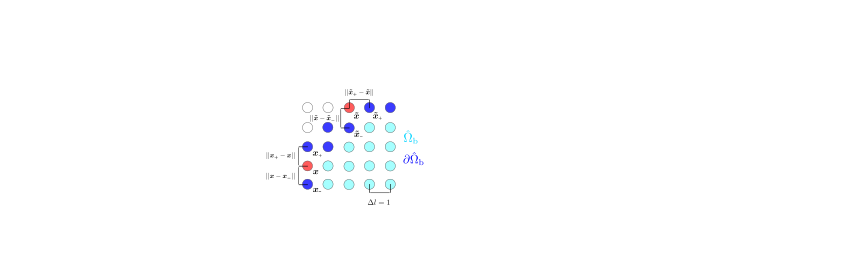
\includegraphics[width=0.5\textwidth, trim={0cm 0cm 0cm 0cm}]{Images/deltas.pdf}
	\vspace{3.8mm}
	\caption{Ilustrace významů a možných pozic bodů $ \vec{x_{-}} $ a $ \vec{x_{+}} $ a znázornění vzdáleností sousedních bodů a jejich vztahu k $ \Delta l $ v námi uvažovaném nastavení. Všechny výrazy v normách budou rovny jedné, proto bude platit pro všechny body $ \Delta s(\vec{x}) = 1 $.}
	\label{fig:deltas}
\end{figure}

Vztah \eqref{eq:sim} se skládá ze dvou hlavních částí, a to z výpočtu úplného tenzoru napětí a z výpočtu normálového vektoru v diskrétním nastavení LBM. Výpočet jednotkového normálového vektoru v~diskrétní mřížce je přímočarý, pokud máme k dispozici analytický popis hranice obtékaného tělesa. Normálový vektor v zadaném bodě pak nalezneme metodami matematické analýzy. V případě, že nemáme k dispozici analytický popis, popíšeme křivku množinou lagrangeovských bodů $ \vec{X} = \vec{X} (s) $, kde $ s $ značí parametrickou souřadnici lagrangeovského bodu. Křivku dále nahradíme po částech lineární aproximací, kdy dva sousední lagrangeovské body spojíme úsečkou. Normálové vektory v bodech podél úsečky pak spočteme jako kolmice na tyto úsečky. Normálové vektory v lagrangeovských bodech určíme jako průměr normálových vektorů ze sousedních lagrangeovských bodů. Konstrukce je schematicky vyobrazena na obr. \ref{fig:curve}.

\begin{figure}[h]
	\centering
	\vspace{2.8mm}
	\includegraphics[width=0.8\textwidth, trim={7.9cm 1.6cm 0cm 0cm}]{Images/lincurve.pdf}
	\vspace{1.8mm}
	\caption{Ilustrace konstrukce normálových vektorů u obecné křivky bez zadaného analytického předpisu. Červené normálové vektory v jednotlivých lagrangeovských bodech vznikly zprůěrováním sousedních černě zbarvených normálových vektorů.}
	\label{fig:curve}
	\vspace{0mm}
\end{figure}
Jako další rozebereme možné způsoby, jak přistoupit k výpočtu  $ \sigma_{ij} $.


\subsubsection{\fontsize{11}{15}\selectfont Aproximace diferencí}
Jako základní aproximaci parciálních derivací ze vztahů \eqref{newton} lze použít náhradu pomocí diference. 
%Definujme bod $ \vec{x^{j}} $ vztahem
%\begin{equation}
%\vec{x^{j}} = \vec{x} + \delta_{1j} \, \Delta t \vec{\xi}_{1} + \delta_{2j}  \, \Delta t \vec{\xi}_{2}, \hspace{1mm} j \in \{1,2\},
%\end{equation}
Uvažujme diferencovatelnou funkci $ g = g(\vec{x}, t) $. Pro jednoduchost označme parciální derivace funkce $ g $ dle patřičných směrů jako
\begin{equation}
\partial_{i}g(\vec{x}, t) \coloneqq \partial_{x_i} g(\vec{x}, t) = \frac{\partial g(\vec{x}, t)}{\partial {x_i}}, \hspace{2mm} i \in \{1,2\}.
\end{equation}
Nechť $ \vec{x} \in \hat{\Omega}_{\mathrm{b}} $. Poté zavádíme pro parciální derivaci ve směru $ {x_i} $ aproximaci
\begin{equation}\label{eq:parc derivace}
\partial_{i} g(\vec{x}, t)\approx
\begin{dcases*}
	\ 0 & \hspace{2mm} pro $ \vec{x} + \Delta t \vec{\xi}_{i} \in \hat{\Omega}_{\mathrm{b}}$, $ \vec{x} - \Delta t \vec{\xi}_{i} \in \hat{\Omega}_{\mathrm{b}}$,\\[3pt]
	\ \dfrac{g (\vec{x}, t) - g (\vec{x} - \Delta t \vec{\xi}_{i}, t)}{\Delta l} & \hspace{2mm} pro $ \vec{x} + \Delta t \vec{\xi}_{i} \in \hat{\Omega}_{\mathrm{b}}$, $ \vec{x} - \Delta t \vec{\xi}_{i} \notin \hat{\Omega}_{\mathrm{b}}$,\\[3pt]
	\ \dfrac{g (\vec{x} + \Delta t \vec{\xi}_{i}, t) - g (\vec{x}, t)}{\Delta l} & \hspace{2mm} pro $ \vec{x} + \Delta t \vec{\xi}_{i} \notin \hat{\Omega}_{\mathrm{b}}$, $ \vec{x} - \Delta t \vec{\xi}_{i} \in \hat{\Omega}_{\mathrm{b}}$,\\[3pt]
	\ \dfrac{g (\vec{x} + \Delta t \vec{\xi}_{i}, t) - g (\vec{x} - \Delta t \vec{\xi}_{i}, t)}{2\Delta l} & \hspace{2mm} pro $ \vec{x} + \Delta t \vec{\xi}_{i} \notin \hat{\Omega}_{\mathrm{b}}$, $ \vec{x} - \Delta t \vec{\xi}_{i} \notin \hat{\Omega}_{\mathrm{b}}$,
\end{dcases*}
\hspace{3mm}
i \in \{1,2\}.
\end{equation}
Volbou $ g = u_1$, resp. $ g = u_2$, pak dostaneme podle vztahu \eqref{eq:parc derivace} aproximace pro parciální derivace $ \partial_{j} u_{i}(\vec{x}, t), \, i,j \in \{1, 2\}$. 
%kde $ \delta_{ij} $ je Kroneckerovo delta. Příklad pozice bodu $ \vec{x^{j}} $ na mřížce je k nahlédnutí na obr. \ref{fig:sim}.

%\begin{figure}[h]
%	\centering
%	\vspace{0.8mm}
%	\includegraphics[width=0.4\textwidth]{Images/simxj.pdf}
%	\vspace{1.8mm}
%	\caption{Ilustrace konstrukce bodů $ \vec{x^{1}} $ a $ \vec{x^{2}} $ potřebných pro dopřednou diferenci a příklady normálových vektorů vyhodnocených v uzlech mřížky, které reprezentují hranici obtékaného tělesa.}
%	\label{fig:sim}
%	\vspace{1.8mm}
%\end{figure}

 V kombinaci se vztahem \eqref{eq:stress_int} a za použití \eqref{eq:parc derivace} platí pro aproximaci dynamického tenzoru napětí
\begin{equation}\label{eq:front difference}
	\sigma^{\, \mu}_{ij} \, (\vec{x}, t) = \mu \, \Bigg( 
%	\frac{\vec{u}_{i} (\vec{x^{j}}, t) - \vec{u}_{i} (\vec{x}, t)}{\Delta l} + \frac{\vec{u}_{j} (\vec{x^{i}}, t) - \vec{u}_{j} (\vec{x}, t)}{\Delta l} 
	\partial_{j} u_{i}(\vec{x}, t) + \partial_{i} u_{j}(\vec{x}, t)
	\Bigg) \: , \hspace{2mm} i,j \in \{1,2\}.
\end{equation}
Pro dynamickou viskozitu $ \mu $ dále platí vztah
\begin{equation}\label{eq:mu}
\mu = \rho \nu,
\end{equation}
můžeme tedy celkem pro úplný tenzor napětí psát
\begin{equation}\label{eq:total stress tensor}
\sigma_{ij} \, (\vec{x}, t) = - \delta_{ij} \, \rho c^{2}_{s} + \sigma^{\, \mu}_{ij} \, (\vec{x}, t) \,, \hspace{2mm} i,j \in \{1,2\},
\end{equation}
kde jsme pro tlak využili vztah \eqref{tlakLBM}.
\subsubsection{\fontsize{11}{15}\selectfont Lokální výpočet}\label{lokalni vypocet}
\section*{\fontsize{11}{15}\selectfont Aproximace dynamického tenzoru napětí}
Z \eqref{eq:BTR} lze pomocí Chapmanova-Enskogova asymptotického rozvoje distribuční funkce určit explicitní vyjádření složek dynamického a úplného tenzoru napětí, viz \cite{Guo}. Buď dále $ \tau $ relaxační čas zavedený v sekci \ref{kol}. Dále definujme rovnovážnou distribuční funkci ve tvaru
\begin{equation}\label{eq:feq}
f^{\mathrm{eq}}_{k} = \rho w_{k} \, \Bigg(1 + \frac{\vec{\xi_{k}} \cdot \vec{u}}{c^{2}_{s}} + \frac{(\vec{\xi_{k}} \cdot \vec{u})^2}{2c^{4}_{s}} - \frac{\vec{u} \cdot \vec{u}}{2c^{2}_{s}} \Bigg)\, , \hspace{2mm} k \in \{0,\dots,q-1\},
\end{equation}
kde $ w_{k} $ představují váhy specifické pro vybraný rychlostní model. Konkrétně pro model D2Q9 platí
\begin{align}\label{weighs}
\begin{split}
w_{0} &  = \dfrac{4}{9},\\[4pt]
w_{1} = w_{2} = w_{3} = w_{4} & = \frac{1}{9},\\[4pt]
w_{5} = w_{6} = w_{7} = w_{8} & = \frac{1}{36}.
\end{split}
\end{align}
Pro dynamický tenzor napětí pak platí vztah
\begin{equation}\label{eq: basic dynamic stress}
\sigma^{\, \mu}_{ij} \, (\vec{x}, t) = \Bigg(1 - \frac{\Delta t}{2 \tau}\Bigg) \, \sum_{k=0}^{q-1}f^{\mathrm{neq}}_{k} (\vec{x}, t) \, {\xi}_{k,1} {\xi}_{k,2},
\end{equation}
kde $ f^{\mathrm{neq}}_{k} $ je nerovnovážná distribuční funkce definovaná jako $ f^{\mathrm{neq}}_{k} = f^{}_{k} - f^{\mathrm{eq}}_{k}$. Úplný tenzor napětí splňuje vztah \eqref{eq:total stress tensor}, kde pro $ \sigma^{\, \mu}_{ij} $ využijeme \eqref{eq: basic dynamic stress}.

\subsubsection*{\fontsize{11}{15}\selectfont Aproximace úplného tenzoru napětí}
Pomocí Chapmanova-Enskogova asymptotického rozvoje je také možné odvodit explicitní vztah přímo pro složky úplného tenzoru napětí. V tomto odvození jsou tedy zahrnuty i diagonální členy obsahující tlak. Pro složky úplného tenzoru dle tohoto odvození platí tvar
\begin{equation}\label{eq:inamuro}
\sigma_{ij} \, (\vec{x}, t) = - \frac{\rho c^{2}_{s}}{2 \tau} \delta_{ij} - \Bigg(1 - \frac{\Delta t}{2 \tau}\Bigg) \, \sum_{k=0}^{q-1}f_{k} ({\xi}_{k,1} - {u}_{1})({\xi}_{k,2} - {u}_{2}),
\end{equation}
detailnější odvození je k nahlédnutí v \cite{Inamuro1997}.
\subsubsection*{\fontsize{11}{15}\selectfont Aproximace úplného tenzoru napětí za použití modifikované rovnovážné funkce}
Poslední model, na jehož základě je odvozen vztah pro výpočet úplného tenzoru napětí, je založen na využití rozdílného tvaru rovnovážné distribuční funkce. V tomto případě je uvažován tvar
\begin{equation}\label{eq:feq suzuki}
f^{\mathrm{eq}}_{k} = w_{k} \, \Bigg(\rho  + \frac{\vec{\xi_{k}} \cdot \vec{u}}{c^{2}_{s}} + \frac{(\vec{\xi_{k}} \cdot \vec{u})^2}{2c^{4}_{s}} - \frac{\vec{u} \cdot \vec{u}}{2c^{2}_{s}} \Bigg).
\end{equation}
Lze ukázat, že při odvození pomocí rovnovážné funkce ve tvaru \eqref{eq:feq suzuki} platí pro úplný tenzor napětí vztah
\begin{equation}\label{eq:suzuki}
\sigma_{ij} \, (\vec{x}, t) = - \frac{\rho c^{2}_{s}}{2 \tau} \delta_{ij} - \Bigg(1 - \frac{\Delta t}{2 \tau}\Bigg) \, \sum_{k=0}^{q-1}f_{k} ({\xi}_{k,1} - {u}_{1})({\xi}_{k,2} - {u}_{2}) - \Big(\frac{3\rho}{c^{2}_{s}} - 1\Big)\,{u}_{1}{u}_{2},
\end{equation}
detaily odvození lze najít v \cite{Suzuki2018}.

\subsubsection{\fontsize{11}{15}\selectfont Označení způsobů výpočtu}\label{oznaceni zpusobu}
V praktické části budeme využívat výše popsané způsoby pro výpočet tenzoru napětí, proto pro snadnější orientaci v textu zavedeme stručná označení pro tyto různé způsoby. Tato označení jsou uvedeny v~tab.~\ref{tab:names of local}. Názvy byly zavedeny dle jmen autorů článků, z kterých byly vztahy pro výpočet převzaty.

\begin{table}[H]
	\vspace{3mm}
	\centering
	\def\arraystretch{1.65}%  1 is the default, change whatever you need
	\begin{tabularx}{0.815\textwidth}{l r}
		\hline
		Název metody výpočtu & Označení \\
		\hline
		Aproximace diferencí 			\		& Diference \\
		Aproximace dynamického tenzoru napětí \cite{NASA} 			\		& Mei \\
		Aproximace úplného tenzoru napětí \cite{Inamuro2000} 	\	& Inamuro \\
		Aproximace úplného tenzoru napětí za použití modifikované $ f^{\mathrm{eq}} \: \cite{Suzuki2018} $  \ & Suzuki \\
		\hline
	\end{tabularx}
	\vspace{5mm}
	\caption{Stručná označení použitých metod lokálního výpočtu tenzoru napětí ze sekce \ref{lokalni vypocet}.}
	\label{tab:names of local}
\end{table}
\vspace{1mm}

\subsection{Počáteční podmínky}\label{initial conditions}
Uvažujme nyní oblast definovanou vztahem \eqref{eq:oblast}. K nastavení počáteční podmínky využijeme rovnovážnou distribuční funkci $ f^{\mathrm{eq}} $. Definujeme počáteční rozložení $ \rho $ a $ \vec{u} $ jako $ \rho _{\mathrm{ini}} $, resp. $ \vec{u} _{\mathrm{ini}} $. Poté pro každý uzel $ \vec{x} \in \hat{\Omega} $ v čase $ t=0 $ bude platit

\begin{equation}\label{eq:initial condition}
f^{}_{k} (\vec{x}, 0) = f^{\mathrm{eq}}_{k} (\rho _{\mathrm{ini}} (\vec{x}), \vec{u} _{\mathrm{ini}} (\vec{x})), \hspace{3mm} k \in \{0, 1, \dots q-1\}.
\end{equation}
Jednoznačnou výhodou tohoto přístupu je jeho malá náročnost na implementaci a čas výpočtu. Nevýhodou je však fakt, že nemusí být zcela konzistentní s předepsanými okrajovými podmínkami, viz \cite{Kruger}.

Existuje i přesnější přístup, jak předepsat počáteční podmínky, např. viz  \cite{Kruger}. Implementačně je však tento přístup složitější, proto bude v této práci pro jednoduchost použit pouze předpis pomocí \eqref{eq:initial condition}.

\subsection{Okrajové podmínky}\label{boundary conditions}
%Při simulování reálného fyzikálního modelu je vhodná volba okrajových podmínek velice důležitá.
V této sekci popíšeme několik okrajových podmínek, které budou následně využity v praktické části této práce.
\subsubsection{\fontsize{12}{15}\selectfont Odtoková okrajová podmínka}\label{bc outlet}
Jako první rozebereme okrajovou podmínku, kterou budeme předepisovat na odtokové části hranice~$ \partial \hat{\Omega}_{\mathrm{out}} $. Podmínku budeme předepisovat v souladu s~\cite{GeierCuLBM} a uvažujeme rychlostní model D2Q9.

Uzly na hranici $ \partial \hat{\Omega}_{\mathrm{out}} $ postrádají uzly, ze kterých by došlo k převzetí hodnoty distribuční funkce ve~směrech $ \vec{\xi_{k}} , k \in \{3,6,7\}$. Jednoduchou metodou, jak tento problém vyřešit a efektivně tak oblast uzavřít, je nahradit chybějící distribuční funkce hodnotami z uzlů z předchozí vrstvy, tj. zkopírovat distribuční funkce z příslušných sousedních uzlů ve směru od hranice do oblasti.

Tato podmínka odpovídá předepsání nulové derivace těchto distribučních funkcí v normálovém~směru $ \vec{n} $ k hranici,tj.~platí
\begin{equation}
\nabla f^{}_{k} \cdot \vec{n} = 0, \hspace{3mm} k \in \{3, 6, 7\},
\end{equation}
kde indexy odpovídají označení rychlostí v obr. \ref{fig:lattice}.
\subsubsection{\fontsize{12}{15}\selectfont Bounce-back okrajová podmínka}
Bounce-back okrajová podmínka patří v LBM k používaným okrajovým podmínkám simulujícím chování tekutiny na hranici s pevnou látkou. Její výhoda je jednoduchost implementace. Na rozhraní tekutiny a rigidní látky předpokládáme neklouzavou (anglicky \textit{no-slip}) okrajovou podmínku, tj. uvažujeme, že je zde rychlost tekutiny nulová. Tento předpoklad bounce-back okrajová podmínka splňuje. Podrobně je tato okrajová podmínka rozebrána v \cite{Kruger}.

Jak název této okrajové podmínky napovídá, její hlavní princip je takový, že uvažujeme odraz hypotetických částic narážejících na rigidní pevnou látku zpět do směrů, ze kterých původně na rozhraní doputovaly. Bounce-back okrajová podmínka může být realizována dvěma různými způsoby, které jsou nazývány:
\begin{itemize}
	\item \textbf{Fullway bounce-back}, při kterém je uvažováno, že hypotetické částice při odrazu doputují až do uzlů pevné látky, kde je jejich směr v dalším kroku šíření obrácen, viz obr. \ref{fig:bbfw},
	\begin{figure}[h]
		\centering
		\vspace{2mm}
		\hspace{7mm}
		\includegraphics[width=0.9\textwidth]{Images/bbfw.pdf}
		\vspace{2.8mm}
		\caption{Schématické znázornění fullway bounce-back okrajové podmínky. Šipky představují směr šíření hypotetické částice, oblast s šedou barvou představuje pevné těleso a čárkovaná hranice odpovídá pozici rozhraní.}
		\label{fig:bbfw}
		\vspace{1.8mm}
	\end{figure}
	\item \textbf{Halfway bounce-back}, při kterém je uvažováno, že hypotetické částice při odrazu doputují pouze do poloviny vzdálenosti mezi uzlem tekutiny a látky, přičemž jejich směr je obrácen během jednoho kroku šíření, viz obr. \ref{fig:bbhw}.
	\begin{figure}[h]
		\centering
		\vspace{2mm}
		\includegraphics[width=0.73\textwidth]{Images/bbhw.pdf}
		\vspace{1.8mm}
		\caption{Schématické znázornění halfway bounce-back okrajové podmínky. Šipky představují směr šíření hypotetické částice, oblast s šedou barvou představuje pevné těleso a čárkovaná hranice odpovídá pozici rozhraní.}
		\label{fig:bbhw}
		\vspace{1.8mm}
	\end{figure}
\end{itemize}
I přesto, že se názvy typů této okrajové podmínky liší, v obou přístupech je uvažováno, že se rozhraní nachází v polovině vzdálenosti mezi uzly tekutiny a pevné látky, viz obr. \ref{fig:staircase}. Tato skutečnost nepůsobí problémy při modelování proudění okolo rovných zdí, které jsou rovnoběžné s použitou mřížkou. Pro zakřivené hranice nerovnoběžné s mřížkou však metoda bounce-back dává za vznik "schodovitému" \ tvaru hranice, a tedy neposkytuje vhodnou aproximaci skutečné pozice rozhraní, viz obr. \ref{fig:staircase}.
\begin{figure}[H]
	\centering
	\vspace{2mm}
	\includegraphics[width=0.37\textwidth]{Images/stairboundary.pdf}
	\vspace{2mm}
	\caption{"Schodovitý" \ tvar hranice vznikající při použití bounce-back okrajové podmínky.}
	\label{fig:staircase}
	\vspace{1.8mm}
\end{figure}

\subsubsection{\fontsize{12}{15}\selectfont Bouzidiho interpolační okrajová podmínka}
Bouzidiho okrajová podmínka uvažující reálný tvar pevné překážky byla poprvé navržena v \cite{Bouzidi2001}. V~tomto schématu je pro výpočet distribuční funkce aplikována interpolace, pro jejíž popis definujme bezrozměrný parametr $ \Theta $ vztahem
\begin{equation}\label{eq:q}
\Theta = \frac{\norm{\vec{x}_{f{_A}}-\vec{x}_w}}{\norm{\vec{x}_{f{_A}}-\vec{x}_b}},
\end{equation}
kde $ \vec{x}_f $ je uzel tekutiny na hranici, $ \vec{x}_b =  \vec{x}_{f{_A}} + \Delta t \vec{\xi_{k}}$ je uzel pevné překážky a dále $ \vec{x}_w$ je bod na reálné hranici objektu tak, jak je ilustrováno na obr. \ref{fig:bouz} a obr. \ref{fig:bouz2}.
\begin{figure}[h]
	\centering
	\vspace{.1mm}
	\includegraphics[width=0.5\textwidth]{Images/bouzidi.pdf}
	\vspace{1.8mm}
	\caption{Schématické znázornění Bouzidiho interpolační podmínky. Černé body na skutečné hranici tělesa (šedá oblast) představují pozice všech bodů $ \vec{x}_w$, které slouží k výpočtu parametru $ \Theta $ pro různé body tekutiny $ \vec{x}_{f{_A}} $ pro různé směry.}
	\label{fig:bouz}
	\vspace{1.8mm}
\end{figure}

\begin{figure}[h]
	\centering
	\vspace{-5.8mm}
	\includegraphics[width=0.85\textwidth]{Images/bouzidi2.pdf}
	\vspace{1.8mm}
	\caption{Ilustrace významu bodů $ \vec{x}_{f{_B}} $ a $ \vec{x}_{f{_C}} $ v jedné dimenzi. Dále je ilustrován význam členů vyskytujících se ve výpočtu parametru $ \Theta $.}
	\label{fig:bouz2}
	\vspace{1.8mm}
\end{figure}
Uvažujme dále nulovou rychlost v hraničních bodech. Tvar pro výpočet distribuční funkce pomocí Bouzidiho schématu závisí na hodnotě parametru $ \Theta $. K odvození můžeme použít lineární nebo kvadratickou interpolaci \cite{Bouzidi2001}.

Při použití lineární interpolace má Bouzidiho okrajová podmínka tvar
\begin{align}\label{eq:lbouz}
\begin{split}
\Theta &< \dfrac{1}{2}: \hspace{7mm} 
f_{\bar{k}}\left(\vec{x}_{f{_A}}, t+\Delta t\right) = 2 \Theta f_{k}^{*}\left(\vec{x}_{f{_A}}, t\right)+(1-2 \Theta) f_{k}^{*}\left(\vec{x}_{f{_B}}, t\right),\\[6pt]
\Theta &\geq \dfrac{1}{2}: \hspace{7mm} f_{\bar{k}}\left(\vec{x}_{f{_A}}, t+\Delta t\right) = \frac{1}{2 \Theta} f_{k}^{*}\left(\vec{x}_{f{_A}}, t\right)+\frac{2 \Theta-1}{2 \Theta} f_{\bar{k}}^{*}\left(\vec{x}_{f{_A}}, t\right),
\end{split}
\end{align}
kde index $ \bar{k} $ splňuje $ \vec{\xi_{\bar{k}}} = -\vec{\xi_{k}}$.

Situace, kdy $ \Theta < 1/2$ může být interpretována tak, že je reálná hranice blíže uzlu pevného tělesa. Naopak pro $ \Theta \geq 1/2$ platí, že je skutečná hranice blíže uzlu tekutiny.

Použitím kvadratické interpolace získáme pro Bouzidiho okrajovou podmínku tvar
\begin{align}\label{eq:qbouz}
\begin{split}
\Theta &< \dfrac{1}{2}: \hspace{3mm} 
f_{\bar{k}}\left(\vec{x}_{f{_A}}, t+\Delta t\right) =
\Theta \left( 1 + 2\Theta \right) f_{k}^{*}\left(\vec{x}_{f{_A}}, t\right)+
(1-4 \Theta^2) f_{k}^{*}\left(\vec{x}_{f{_B}}, t\right)-
\Theta \left( 1 - 2\Theta \right) f_{k}^{*}\left(\vec{x}_{f{_C}}, t\right),\\[6pt]
\Theta &\geq \dfrac{1}{2}: \hspace{3mm}
f_{\bar{k}}\left(\vec{x}_{f{_A}}, t+\Delta t\right) =
\frac{1}{\Theta \left(2 \Theta + 1\right)} f_{k}^{*}\left(\vec{x}_{f{_A}}, t\right) +
\frac{2\Theta - 1}{\Theta} f_{\bar{k}}^{*}\left(\vec{x}_{f{_A}}, t\right) -
\frac{2\Theta - 1}{2 \Theta + 1} f_{\bar{k}}^{*}\left(\vec{x}_{f{_B}}, t\right),
\end{split}
\end{align}
kde význam bodu $ \vec{x}_{f{_C}} $ je ilustrován na obr. \ref{fig:bouz2}.

Je snadné nahlédnout, že Bouzidiho okrajová podmínka zobecňuje halfway bounce-back podmínku, pro kterou by platilo $ \Theta = 1/2$.


\subsubsection{\fontsize{12}{15}\selectfont Sjednocená interpolační okrajová podmínka}
Bouzidiho interpolační schéma používá dva různé vzorce na základě hodnoty parametru $ \Theta $. V \cite{Yu2003} však bylo odvozeno interpolační schéma, které oba případy sjednocuje v jeden společný tvar pro všechny hodnoty~$ \Theta $. Opět lze pro jeho odvození využít lineární nebo kvadratickou interpolaci.
Při použití lineární interpolace má tato sjednocená okrajová podmínka tvar
\begin{equation}\label{eq:luni}
f_{\bar{k}}\left(\vec{x}_{f{_A}}, t+\Delta t\right)= \frac{1}{1+\Theta} \, \Big[ \Theta f_{k}\left(\vec{x}_{f{_A}}, t\right)+(1-\Theta) {f}_{k}\left(\vec{x}_{f{_B}}, t\right) +\Theta {f}_{\bar{k}}\left(\vec{x}_{f{_A}}, t\right) \Big].
\end{equation}
Použitím kvadratické interpolace získáme pro sjednocenou okrajovou podmínku tvar
\begin{align}\label{eq:quni}
\begin{split}
f_{\bar{k}}\left(\vec{x}_{f}, t+\Delta t\right)=& \,
\frac{1}{(1+\Theta)(2+\Theta)} \, \Big[\Theta(1+\Theta) {f}_{k}\left(\vec{x}_{f{_A}}, t\right)+2\left(1-\Theta^{2}\right) {f}_{k}\left(\vec{x}_{f{_B}}, t\right)
\\&-\Theta(1-\Theta) {f}_{k}\left(\vec{x}_{f{_C}}, t\right)+2 \Theta(2+\Theta) {f}_{\bar{k}}\left(\vec{x}_{f{_A}}, t\right) 
-\Theta(1+\Theta) {f}_{\bar{k}}\left(\vec{x}_{f{_B}}, t\right) \Big].
\end{split}\end{align}
\subsubsection{\fontsize{12}{15}\selectfont Označení okrajových podmínek}
V praktické části budeme testovat jednotlivé okrajové podmínky popsané v rámci této kapitoly. Bude zkoumán jejich vliv při předepsání na hranici obtékaného tělesa. Proto podobně jako pro různé způsoby výpočtu tenzoru napětí zavedeme pro pozdější snazší orientaci v textu stručná označení testovaných podmínek podle tab. \ref{tab:names of bc}.
\begin{table}[H]
	\vspace{2mm}
	\centering
	\def\arraystretch{1.65}%  1 is the default, change whatever you need
	\begin{tabularx}{0.75\textwidth}{l r}
		\hline
		Název okrajové podmínky & Označení \\
		\hline
		Full-way bounce-back okrajová podmínka 			\		& Bounce-back \\
		Bouzidiho okrajová podmínka s lineární interpolací 	\	& Bouzidi 1 \\
		Bouzidiho okrajová podmínka s kvadratickou interpolací \ & Bouzidi 2	 \\
		Sjednocená okrajová podmínka s lineární interpolací \	& Sjednocená 1 \\
		Sjednocená okrajová podmínka s kvadratickou interpolací \ & Sjednocená 2 \\
		\hline
	\end{tabularx}
	\vspace{1mm}
	\caption{Stručná označení použitých okrajových podmínek ze sekce \ref{boundary conditions} testovaných na hranici obtékaného tělesa.}
	\label{tab:names of bc}
\end{table}

\vspace{-2mm}
\subsection{Algoritmus LBM}\label{algo}
V několika krocích nyní shrneme samotný algoritmus LBM. Vývojový diagram algoritmu je k nahlédnutí na obr. \ref{fig:algo}.
\begin{enumerate}
	\item \textbf{Inicializace:} Nastavení počátečních podmínek v mřížce, viz sekce \ref{initial conditions}.
	\item \textbf{Cyklus:} Kroky se opakují, dokud není splněna podmínka ukončení, která je zadána uživatelem.
	\begin{enumerate}
		\item \textbf{Šíření:} Propagace postkolizních distribučních funkcí $ f^{*}_{k} $  v příslušných směrech $ \vec{\xi_{k}} $.
		\item \textbf{Výpočet hodnot makroskopických veličin:} Výpočet makroskopických veličin pomocí vztahů \eqref{macroeq}.
		\item \textbf{Kolize:} Výpočet postkolizního stavu distribuční funkce pomocí \eqref{eq:collision}.
		\item \textbf{Řešení okrajových podmínek:} Řešení okrajových podmínek diskutovaných v sekci \ref{boundary conditions}.
	\end{enumerate}
	\item \textbf{Konec algoritmu.}
\end{enumerate}
\begin{figure}[H]
	\centering
	\vspace{-8mm}
	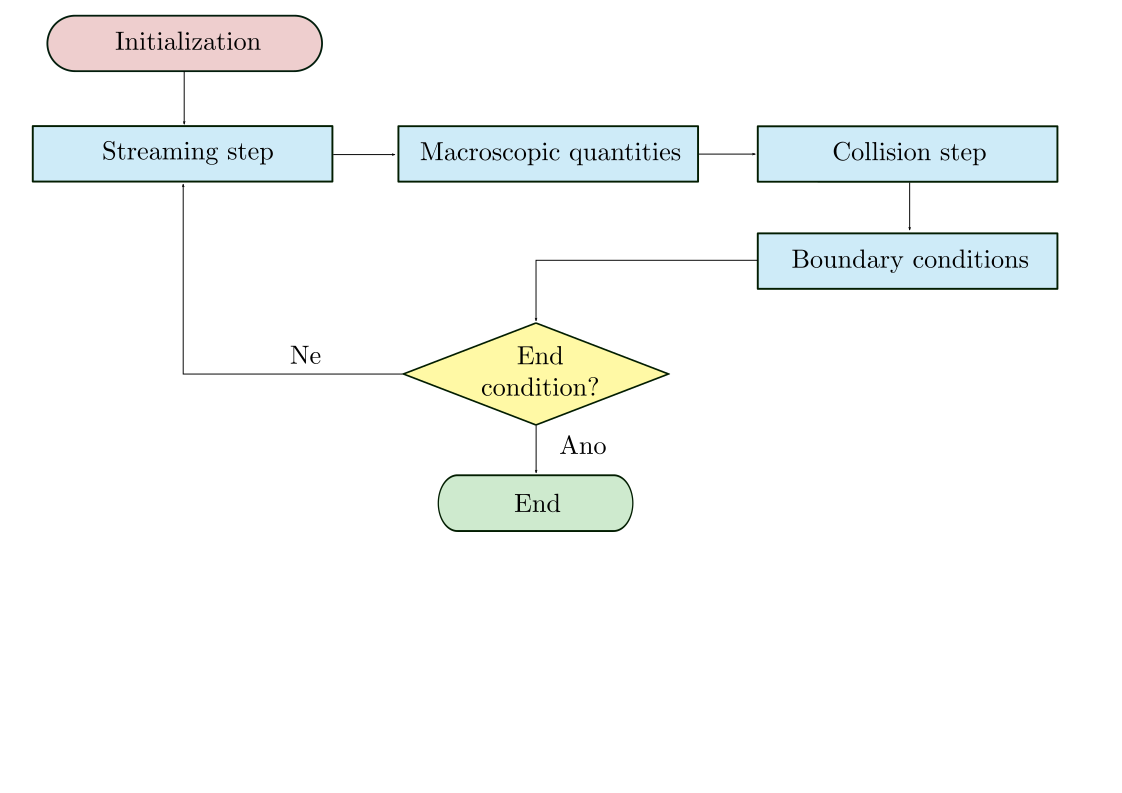
\includegraphics[width=0.35\textwidth]{Images/algo.pdf}
	\caption{Vývojový diagram algoritmu LBM.}
	\label{fig:algo}
\end{figure}

\section{Poznámky k implementaci}\label{implementace}
V této sekci popíšeme některé části kódu, které byly v rámci této práce implementovány. Nejprve rozebereme obecnou strukturu kódu a popíšeme generátor vstupních dat, který byl v rámci práce implementovaný. Následně popíšeme příklad realizace jedné z interpolačních okrajových podmínek popsaných v sekci \ref{boundary conditions}.
\subsection{Generování vstupních dat a struktura kódu}\label{data}
V rámci této práce budeme uvažovat pouze úlohy, ve kterých je hranice obtékaného tělesa nepohyblivá. Veškeré charakteristiky týkající se geometrie lze pak určit již před samotným spuštěním simulace. Z tohoto důvodu bylo navrženo schéma, ve kterém jsou nejprve vygenerovaná vstupní data nutná pro simulaci a až následně jsou spuštěny samotné numerické výpočty využívající tato data. Úloha je popsána uživatelem pomocí parametrů, kterými jsou rozměry výpočetní oblasti a rozlišení diskrétní mřížky využité v LBM.

V programovacím jazyce Python byl implementován modul $\mathtt{DataGenerator} $, který obsahuje třídy reprezentující různé geometrické objekty, které je možné následně v numerické simulaci využít. Jmenovitě byly implementovány následující třídy:
\begin{itemize}
	\item $\mathtt{Line} $ - třída reprezentující úsečku,
	\item $\mathtt{Polygon} $ - třída reprezentující pravidelný mnohoúhelník,
	\item $\mathtt{Circle} $ - třída reprezentující kruh,
	\item $\mathtt{SVGCurve} $ - třída reprezentující křivku, která byla vytvořena ve formátu $\mathtt{SVG} $ (z anglického \textit{Scalable Vector Graphics} \cite{Eisenberg2002}).
\end{itemize}
Pro generování úseček při práci se třídami $\mathtt{Line} $, $\mathtt{Polygon} $ a $\mathtt{SVGCurve} $ byl bez použití externích knihoven implementován Bresenhamův algoritmus \cite{Bresenham}. Tento algoritmus patří k základním algoritmům pro vykreslování úseček do rastrové mřížky a byl zvolen za účelem dosáhnutí co nejvíce přesné projekce objektu na diskrétní mřížku. Různé geometrické útvary, které je možné generovat, jsou k nahlédnutí na obr. \ref{fig:geometrie}.

\begin{figure}[H]
	\centering
	\vspace{2mm}
	\includegraphics[width=0.8\textwidth]{Images/geometrie.png}
	\vspace{3mm}
	\caption{Příklady objektů, které lze generovat a následně využít v numerické simulaci. Vizualizace simulace je realizována pomocí knihovny SDL. Barevná škála vyjadřuje velikost rychlosti (od červené barvy po modrou) tekutiny, která dané objekty obtéká jako řešení LBM.}
	\label{fig:geometrie}
\end{figure}

V rámci generování vstupních dat je nejprve každému uzlu mřížky přiřazen jeho typ. Rozlišujeme mezi typy reprezentující tekutinu, hranici tělesa a vrstvu uzlů tělesa bezprostředně sousedících s jeho hranicí. U tříd $\mathtt{Polygon} $ a $\mathtt{Circle} $ zavádíme dále typ uzlu reprezentující vnitřek tělesa. V uzlech hranice tělesa jsou poté vypočteny veličiny, které mohou být použity pro výpočet síly pomocí metody integrace tenzoru napětí a při výpočtu interpolačních okrajových podmínek, tj. jednotkové normálové vektory a~parametry $ \Theta $, viz \eqref{eq:q}. Výpočet parametru $ \Theta $ je blíže rozebrán v sekci \ref{implementace interpolace}.

Pro každý uzel mřížky jsou následně jeho typ, hodnoty normálového vektoru a hodnoty parametru~$ \Theta $ uloženy do textového souboru $\mathtt{input\_data} $. Tento soubor je dále předán programu realizujícímu numerický výpočet dané úlohy pomocí LBM. Jak již bylo zmíněno v úvodu práce, pro numerické řešení byl využit kód vyvíjený na katedře matematiky FJFI ČVUT v Praze, který slouží k řešení Navierových-Stokesových rovnic pro newtonovskou nestlačitelnou tekutinu. Program je implementovaný v jazyce C++ a využívá paralelizace na GPU s využítím platformy CUDA. V kódu jsou jako typy LBM implementovány varianty CLBM a SRT. Pro účely této práce byla v kódu provedena řada úprav, zejména pak:
\begin{itemize}
	\item implementace metody integrace tenzoru napětí pro výpočet síly pomocí diference,
	\item implementace různých způsobů lokálního výpočtu tenzoru napětí,
	\item implementace interpolačních okrajových podmínek,
	\item výpočet sledovaných veličin a jejich následný výpis do souborů.
\end{itemize}
Schéma kódu je k nahlédnutí na obr. \ref{fig:schemakodu}.

\begin{figure}[h]
	\centering
	\vspace{4mm}
	\includegraphics[width=0.55\textwidth]{Images/schemakodu.pdf}
	\caption{Schéma ilustrující propojení modulu $\mathtt{DataGenerator} $ a programu, který realizuje numerický výpočet pomocí LBM.}
	\vspace{2.5mm}
	\label{fig:schemakodu}
\end{figure}

\subsection{Implementace interpolačních okrajových podmínek}\label{implementace interpolace}
V této sekci popíšeme, jakým způsobem byly implementovány interpolační okrajové podmínky popsané v sekci \ref{boundary conditions}. Postup popíšeme pro Bouzidiho okrajovou podmínku s lineární interpolací, analogicky však byly řešeny i ostatní okrajové podmínky, které všechny používají hodnoty parametru $ \Theta $, viz~\eqref{eq:q}. Popíšeme nejdříve výpočet tohoto parametru.

Uvažujme těleso $ {\Omega}_{\mathrm{b}} $ obtékané tekutinou. Parametr $ \Theta $ je nutné vypočítat ve všech bodech $ \vec{x} \in \partial \hat{\Omega}_{\mathrm{b}} $. V každém takovém bodě je pak nutné vypočítat hodnotu $ \Theta $ pro každý ze směrů možného šíření kromě směru odpovídajícímu $ \vec{\xi}_0 $. V rámci modelu D2Q9 tedy celkem určujeme 8 hodnot pro každý bod hranice, označme je $ \Theta_1, \Theta_2, \dots, \Theta_8$, kde číslo indexu odpovídá příslušnému směru, viz obr. \ref{fig:lattice2}. Zdůrazněme, že průsečík $ \vec{x}_w $ s hranicí nemůže existovat pro každý ze směrů (viz obr. \ref{fig:bouz}). Ve směrech, pro které tento průsečík neexistuje, parametr $ \Theta _i $ nedefinujeme a provádíme v nich standardní šíření z okolních uzlů. Z implementačních důvodů pro tyto směry pokládáme  $ \Theta_i = -1$.

Pro určitost dále uvažujme, že v daném směru průsečík $ \vec{x}_w $ existuje, a že analytický popis hranice obtékaného tělesa $ \partial {\Omega}_{\mathrm{b}} $ splňuje vazbu
\begin{equation}\label{eq:kruznice}
	\phi \, (\vec{x}) = 0, \hspace{3mm} \forall \vec{x} \in \partial {\Omega}_{\mathrm{b}}.
\end{equation}

S použitím značení z obr. \ref{fig:bouz} parametrizujme úsečku spojující body $ \vec{x}_{f{_A}} = (x_{f{_A}}, y_{f{_A}})$ a $ \vec{x}_b  = (x_b, y_b)$ jako
\begin{align}\label{eq:parametrizace usecky}
\begin{split}
x=& s \, x_{f{_A}} + (1 - s) \, x_b,
\\
y=& s \, y_{f{_A}} + (1 - s) \, y_b ,
\end{split}
\end{align}
kde $ s \in \langle 0, 1 \rangle $. Dále dosazením \eqref{eq:parametrizace usecky} do rovnice vazby \eqref{eq:kruznice} získáme hodnotu $ s $. Je snadné nahlédnout, že získaná hodnota $ s $ odpovídá hledané hodnotě parametru $ \Theta_i $, a není tedy nutné explicitně počítat souřadnice bodu  $ \vec{x}_w $ a použít vztah \eqref{eq:q}. 

Výše popsaný postup lze využít pro libovolný tvar hranice popsaný vazbou, přičemž v rámci implementace musí být tato vazba explicitně určená. V úlohách v kapitole \ref{vysledky} za vazbu $ \phi $ volíme rovnici kružnice.

Jak již bylo zmíněno, v rámci implementace jsme pro směry, pro které neexistuje průsečík s hranicí, položili $ \Theta_i = -1$. Dále jsme hodnotu $ \Theta_i$ použili k určení typu šíření v daném směru. Pro $ \Theta_i < 0$, tj.~$ \Theta_i = -1$, provádíme standardní šíření, pro hodnoty $ 0 \leq \Theta_i \leq 1 $ pak zvolíme vzorec na základě hodnoty $ \Theta_i $ v souladu se vztahy pro Bouzidiho okrajovou podmínku. Funkce $\mathtt{f\_bouzidi\_1} $, která realizuje Bouzidiho okrajovou podmínku s lineární interpolací, je k nahlédnutí v příkladu kódu \ref{lst:label}. Podotkněme, že v příkladu kódu \ref{lst:label} označuje $ (x_s, y_s) $ bod, ze kterého by do bodu $ \vec{x}_{f{_A}} $ bylo provedeno standardní šíření v příslušném směru. Dále metoda $\mathtt{SD.cdf()} $ slouží k získání hodnoty postkolizní distribuční funkce pro daný směr a uzel. Zbylé části kódu odpovídají značení ze vztahu pro Bouzidiho okrajovou podmínku \eqref{eq:lbouz}.
%\lstinputlisting[language=C++]{fbouzidi.cpp}
\vspace{3mm}
\begin{lstlisting}[caption={Funkce realizující Bouzidiho okrajovou podmínku s lineární interpolací.},label={lst:label},language=C++]
	template< typename LBM_DATA >
	CUDA_HOSTDEV static dreal f_bouzidi_1( LBM_DATA &SD, dreal theta, int k,
		int kpruh, didx xfA, didx yfA, didx xfB, didx yfB, didx xs, didx ys )
	{
 	   // Standardni sireni:
 	   if (theta < 0) {
 					return SD.cdf( kpruh, xs, ys );
	   }
	   // Bouzidi pro theta < 0.5, (2.54):
	   else if (theta < 0.5) {
   				return (1.0 - 2.0 * theta) * SD.cdf( k, xfB, yfB ) + 
   				    	 (2.0 * theta) * SD.cdf( k, xfA, yfA );
	   }
	   // Bouzidi pro theta >= 0.5, (2.54):
	   else {
					return (1.0 - 0.5 / theta) * SD.cdf( kpruh, xfA, yfA ) +
	      		 	   (0.5 / theta) * SD.cdf( k, xfA, yfA );
	   }
	}
\end{lstlisting}